\documentclass[twoside]{book}

% Packages required by doxygen
\usepackage{fixltx2e}
\usepackage{calc}
\usepackage{doxygen}
\usepackage[export]{adjustbox} % also loads graphicx
\usepackage{graphicx}
\usepackage[utf8]{inputenc}
\usepackage{makeidx}
\usepackage{multicol}
\usepackage{multirow}
\PassOptionsToPackage{warn}{textcomp}
\usepackage{textcomp}
\usepackage[nointegrals]{wasysym}
\usepackage[table]{xcolor}

% NLS support packages
\usepackage[T2A]{fontenc}
\usepackage[russian]{babel}

% Font selection
\usepackage[T1]{fontenc}
\usepackage[scaled=.90]{helvet}
\usepackage{courier}
\usepackage{amssymb}
\usepackage{sectsty}
\renewcommand{\familydefault}{\sfdefault}
\allsectionsfont{%
  \fontseries{bc}\selectfont%
  \color{darkgray}%
}
\renewcommand{\DoxyLabelFont}{%
  \fontseries{bc}\selectfont%
  \color{darkgray}%
}
\newcommand{\+}{\discretionary{\mbox{\scriptsize$\hookleftarrow$}}{}{}}

% Page & text layout
\usepackage{geometry}
\geometry{%
  a4paper,%
  top=2.5cm,%
  bottom=2.5cm,%
  left=2.5cm,%
  right=2.5cm%
}
\tolerance=750
\hfuzz=15pt
\hbadness=750
\setlength{\emergencystretch}{15pt}
\setlength{\parindent}{0cm}
\setlength{\parskip}{3ex plus 2ex minus 2ex}
\makeatletter
\renewcommand{\paragraph}{%
  \@startsection{paragraph}{4}{0ex}{-1.0ex}{1.0ex}{%
    \normalfont\normalsize\bfseries\SS@parafont%
  }%
}
\renewcommand{\subparagraph}{%
  \@startsection{subparagraph}{5}{0ex}{-1.0ex}{1.0ex}{%
    \normalfont\normalsize\bfseries\SS@subparafont%
  }%
}
\makeatother

% Headers & footers
\usepackage{fancyhdr}
\pagestyle{fancyplain}
\fancyhead[LE]{\fancyplain{}{\bfseries\thepage}}
\fancyhead[CE]{\fancyplain{}{}}
\fancyhead[RE]{\fancyplain{}{\bfseries\leftmark}}
\fancyhead[LO]{\fancyplain{}{\bfseries\rightmark}}
\fancyhead[CO]{\fancyplain{}{}}
\fancyhead[RO]{\fancyplain{}{\bfseries\thepage}}
\fancyfoot[LE]{\fancyplain{}{}}
\fancyfoot[CE]{\fancyplain{}{}}
\fancyfoot[RE]{\fancyplain{}{\bfseries\scriptsize Создано системой Doxygen }}
\fancyfoot[LO]{\fancyplain{}{\bfseries\scriptsize Создано системой Doxygen }}
\fancyfoot[CO]{\fancyplain{}{}}
\fancyfoot[RO]{\fancyplain{}{}}
\renewcommand{\footrulewidth}{0.4pt}
\renewcommand{\chaptermark}[1]{%
  \markboth{#1}{}%
}
\renewcommand{\sectionmark}[1]{%
  \markright{\thesection\ #1}%
}

% Indices & bibliography
\usepackage{natbib}
\usepackage[titles]{tocloft}
\setcounter{tocdepth}{3}
\setcounter{secnumdepth}{5}
\makeindex

% Hyperlinks (required, but should be loaded last)
\usepackage{ifpdf}
\ifpdf
  \usepackage[pdftex,pagebackref=true]{hyperref}
\else
  \usepackage[ps2pdf,pagebackref=true]{hyperref}
\fi
\hypersetup{%
  colorlinks=true,%
  linkcolor=blue,%
  citecolor=blue,%
  unicode%
}

% Custom commands
\newcommand{\clearemptydoublepage}{%
  \newpage{\pagestyle{empty}\cleardoublepage}%
}

\usepackage{caption}
\captionsetup{labelsep=space,justification=centering,font={bf},singlelinecheck=off,skip=4pt,position=top}

%===== C O N T E N T S =====

\begin{document}

% Titlepage & ToC
\hypersetup{pageanchor=false,
             bookmarksnumbered=true,
             pdfencoding=unicode
            }
\pagenumbering{alph}
\begin{titlepage}
\vspace*{7cm}
\begin{center}%
{\Large C\+S\+V-\/\+S\+Q\+L-\/\+Converter }\\
\vspace*{1cm}
{\large Создано системой Doxygen 1.8.14}\\
\end{center}
\end{titlepage}
\clearemptydoublepage
\pagenumbering{roman}
\tableofcontents
\clearemptydoublepage
\pagenumbering{arabic}
\hypersetup{pageanchor=true}

%--- Begin generated contents ---
\chapter{C\+S\+V-\/\+S\+Q\+L-\/\+Converter}
\label{md__r_e_a_d_m_e}
\Hypertarget{md__r_e_a_d_m_e}
Конвертер csv$<$-\/$>$sqlite 
\chapter{Иерархический список классов}
\section{Иерархия классов}
Иерархия классов.\begin{DoxyCompactList}
\item Q\+Abstract\+Table\+Model\begin{DoxyCompactList}
\item \contentsline{section}{Data\+Table}{\pageref{class_data_table}}{}
\end{DoxyCompactList}
\item Q\+Main\+Window\begin{DoxyCompactList}
\item \contentsline{section}{Main\+Window}{\pageref{class_main_window}}{}
\end{DoxyCompactList}
\end{DoxyCompactList}

\chapter{Алфавитный указатель классов}
\section{Классы}
Классы с их кратким описанием.\begin{DoxyCompactList}
\item\contentsline{section}{\mbox{\hyperlink{class_data_table}{Data\+Table}} \\*Класс \mbox{\hyperlink{class_data_table}{Data\+Table}}. Основной класс в этом проекте }{\pageref{class_data_table}}{}
\item\contentsline{section}{\mbox{\hyperlink{class_main_window}{Main\+Window}} }{\pageref{class_main_window}}{}
\end{DoxyCompactList}

\chapter{Список файлов}
\section{Файлы}
Полный список документированных файлов.\begin{DoxyCompactList}
\item\contentsline{section}{\mbox{\hyperlink{datatable_8cpp}{datatable.\+cpp}} \\*Файл исходников с реализацией всех необходимых функций }{\pageref{datatable_8cpp}}{}
\item\contentsline{section}{\mbox{\hyperlink{datatable_8h}{datatable.\+h}} \\*Заголовочный файл с описанием основного класса проекта }{\pageref{datatable_8h}}{}
\item\contentsline{section}{\mbox{\hyperlink{mainwindow_8cpp}{mainwindow.\+cpp}} \\*Файл исходников с описанием работы главного окна проекта }{\pageref{mainwindow_8cpp}}{}
\item\contentsline{section}{\mbox{\hyperlink{mainwindow_8h}{mainwindow.\+h}} \\*Заголовочный файл с описанием главного окна проекта }{\pageref{mainwindow_8h}}{}
\end{DoxyCompactList}

\chapter{Классы}
\hypertarget{class_data_table}{}\section{Класс Data\+Table}
\label{class_data_table}\index{Data\+Table@{Data\+Table}}


Класс \mbox{\hyperlink{class_data_table}{Data\+Table}}. Основной класс в этом проекте.  




{\ttfamily \#include $<$datatable.\+h$>$}

Граф наследования\+:Data\+Table\+:\begin{figure}[H]
\begin{center}
\leavevmode
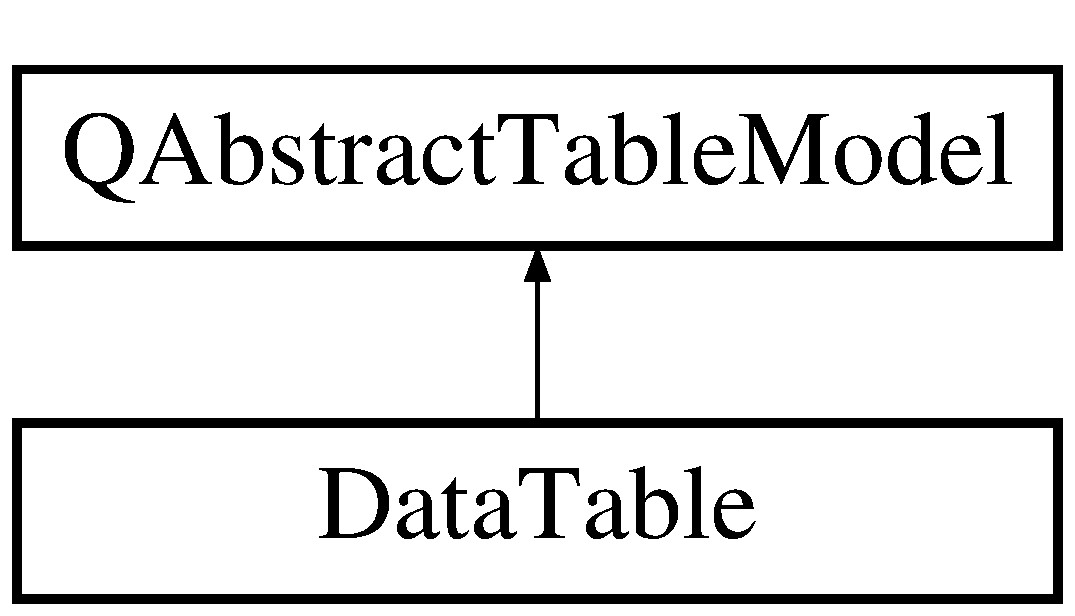
\includegraphics[height=2.000000cm]{class_data_table}
\end{center}
\end{figure}
\subsection*{Открытые члены}
\begin{DoxyCompactItemize}
\item 
\mbox{\hyperlink{class_data_table_a639ccb380db236e70c17de76c05c67f2}{Data\+Table}} (Q\+Object $\ast$parent=nullptr)
\begin{DoxyCompactList}\small\item\em Основной конструктор. \end{DoxyCompactList}\item 
\mbox{\hyperlink{class_data_table_a91add7552f26453ea7d378a1ec24cd2a}{Data\+Table}} (Q\+List$<$ Q\+String $>$ Col\+Name, Q\+List$<$ Q\+String $>$ Data\+Type, Q\+List$<$ Q\+List$<$ Q\+String $>$$>$ Data)
\begin{DoxyCompactList}\small\item\em Конструктор с параметрами. \end{DoxyCompactList}\item 
\mbox{\Hypertarget{class_data_table_a6f97f5c8d7fe892732d34945514c6c5d}\label{class_data_table_a6f97f5c8d7fe892732d34945514c6c5d}} 
void \mbox{\hyperlink{class_data_table_a6f97f5c8d7fe892732d34945514c6c5d}{Type\+Id}} ()
\begin{DoxyCompactList}\small\item\em Функция определения типа данных \end{DoxyCompactList}\item 
void \mbox{\hyperlink{class_data_table_af46ecb3f9f33e2a34ec9866991cd12ff}{Load\+Csv}} (Q\+String filename)
\begin{DoxyCompactList}\small\item\em Чтение файла .csv. \end{DoxyCompactList}\item 
void \mbox{\hyperlink{class_data_table_afb7a2b7446f518aa5fe208dc6df1f686}{Save\+Csv}} (Q\+String filename)
\begin{DoxyCompactList}\small\item\em Запись в файл .csv. \end{DoxyCompactList}\item 
void \mbox{\hyperlink{class_data_table_ab9cbaf9a296c84eb4c969870d83a6555}{Load\+Sql}} (Q\+String filename, Q\+String tablename)
\begin{DoxyCompactList}\small\item\em Чтение файла .db. \end{DoxyCompactList}\item 
void \mbox{\hyperlink{class_data_table_a73852c3ab4dfd0fdc6ce5e99c860824f}{Save\+Sql}} (Q\+String filename, Q\+String tablename)
\begin{DoxyCompactList}\small\item\em Запись в файл .db. \end{DoxyCompactList}\item 
\mbox{\Hypertarget{class_data_table_a4e6651b3d147f8aa796195db5cb5b4db}\label{class_data_table_a4e6651b3d147f8aa796195db5cb5b4db}} 
virtual int {\bfseries row\+Count} (const Q\+Model\+Index \&parent) const override
\item 
\mbox{\Hypertarget{class_data_table_af9507f1dc84206a4961eee8580bbdb49}\label{class_data_table_af9507f1dc84206a4961eee8580bbdb49}} 
virtual int {\bfseries column\+Count} (const Q\+Model\+Index \&parent) const override
\item 
\mbox{\Hypertarget{class_data_table_a095037439684a30c1eb8d34d0c8a118e}\label{class_data_table_a095037439684a30c1eb8d34d0c8a118e}} 
virtual Q\+Variant {\bfseries data} (const Q\+Model\+Index \&index, int role) const override
\item 
\mbox{\Hypertarget{class_data_table_a3a99f20f29c49bde6cf4c43e60422692}\label{class_data_table_a3a99f20f29c49bde6cf4c43e60422692}} 
virtual Q\+Variant {\bfseries header\+Data} (int section, Qt\+::\+Orientation orientation, int role) const override
\end{DoxyCompactItemize}
\subsection*{Друзья}
\begin{DoxyCompactItemize}
\item 
bool \mbox{\hyperlink{class_data_table_a448d6b5189991394bc06db5950f2c8dc}{operator==}} (const \mbox{\hyperlink{class_data_table}{Data\+Table}} \&L, const \mbox{\hyperlink{class_data_table}{Data\+Table}} \&R)
\begin{DoxyCompactList}\small\item\em Сравнение двух переменных класса \mbox{\hyperlink{class_data_table}{Data\+Table}}. \end{DoxyCompactList}\end{DoxyCompactItemize}


\subsection{Подробное описание}
Класс \mbox{\hyperlink{class_data_table}{Data\+Table}}. Основной класс в этом проекте. 

\subsection{Конструктор(ы)}
\mbox{\Hypertarget{class_data_table_a639ccb380db236e70c17de76c05c67f2}\label{class_data_table_a639ccb380db236e70c17de76c05c67f2}} 
\index{Data\+Table@{Data\+Table}!Data\+Table@{Data\+Table}}
\index{Data\+Table@{Data\+Table}!Data\+Table@{Data\+Table}}
\subsubsection{\texorpdfstring{Data\+Table()}{DataTable()}\hspace{0.1cm}{\footnotesize\ttfamily [1/2]}}
{\footnotesize\ttfamily Data\+Table\+::\+Data\+Table (\begin{DoxyParamCaption}\item[{Q\+Object $\ast$}]{parent = {\ttfamily nullptr} }\end{DoxyParamCaption})}



Основной конструктор. 


\begin{DoxyParams}{Аргументы}
{\em parent} & \\
\hline
\end{DoxyParams}
\mbox{\Hypertarget{class_data_table_a91add7552f26453ea7d378a1ec24cd2a}\label{class_data_table_a91add7552f26453ea7d378a1ec24cd2a}} 
\index{Data\+Table@{Data\+Table}!Data\+Table@{Data\+Table}}
\index{Data\+Table@{Data\+Table}!Data\+Table@{Data\+Table}}
\subsubsection{\texorpdfstring{Data\+Table()}{DataTable()}\hspace{0.1cm}{\footnotesize\ttfamily [2/2]}}
{\footnotesize\ttfamily Data\+Table\+::\+Data\+Table (\begin{DoxyParamCaption}\item[{Q\+List$<$ Q\+String $>$}]{Col\+Name,  }\item[{Q\+List$<$ Q\+String $>$}]{Data\+Type,  }\item[{Q\+List$<$ Q\+List$<$ Q\+String $>$$>$}]{Data }\end{DoxyParamCaption})}



Конструктор с параметрами. 


\begin{DoxyParams}{Аргументы}
{\em Col\+Name} & Имена столбцов \\
\hline
{\em Data\+Type} & Типы данных \\
\hline
{\em Data} & Основные данные таблицы \\
\hline
\end{DoxyParams}


\subsection{Методы}
\mbox{\Hypertarget{class_data_table_af46ecb3f9f33e2a34ec9866991cd12ff}\label{class_data_table_af46ecb3f9f33e2a34ec9866991cd12ff}} 
\index{Data\+Table@{Data\+Table}!Load\+Csv@{Load\+Csv}}
\index{Load\+Csv@{Load\+Csv}!Data\+Table@{Data\+Table}}
\subsubsection{\texorpdfstring{Load\+Csv()}{LoadCsv()}}
{\footnotesize\ttfamily void Data\+Table\+::\+Load\+Csv (\begin{DoxyParamCaption}\item[{Q\+String}]{filename }\end{DoxyParamCaption})}



Чтение файла .csv. 


\begin{DoxyParams}{Аргументы}
{\em filename} & Имя файла \\
\hline
\end{DoxyParams}
\mbox{\Hypertarget{class_data_table_ab9cbaf9a296c84eb4c969870d83a6555}\label{class_data_table_ab9cbaf9a296c84eb4c969870d83a6555}} 
\index{Data\+Table@{Data\+Table}!Load\+Sql@{Load\+Sql}}
\index{Load\+Sql@{Load\+Sql}!Data\+Table@{Data\+Table}}
\subsubsection{\texorpdfstring{Load\+Sql()}{LoadSql()}}
{\footnotesize\ttfamily void Data\+Table\+::\+Load\+Sql (\begin{DoxyParamCaption}\item[{Q\+String}]{filename,  }\item[{Q\+String}]{tablename }\end{DoxyParamCaption})}



Чтение файла .db. 


\begin{DoxyParams}{Аргументы}
{\em filename} & Имя файла \\
\hline
{\em tablename} & Имя таблицы \\
\hline
\end{DoxyParams}
\mbox{\Hypertarget{class_data_table_afb7a2b7446f518aa5fe208dc6df1f686}\label{class_data_table_afb7a2b7446f518aa5fe208dc6df1f686}} 
\index{Data\+Table@{Data\+Table}!Save\+Csv@{Save\+Csv}}
\index{Save\+Csv@{Save\+Csv}!Data\+Table@{Data\+Table}}
\subsubsection{\texorpdfstring{Save\+Csv()}{SaveCsv()}}
{\footnotesize\ttfamily void Data\+Table\+::\+Save\+Csv (\begin{DoxyParamCaption}\item[{Q\+String}]{filename }\end{DoxyParamCaption})}



Запись в файл .csv. 


\begin{DoxyParams}{Аргументы}
{\em filename} & Имя файла \\
\hline
\end{DoxyParams}
\mbox{\Hypertarget{class_data_table_a73852c3ab4dfd0fdc6ce5e99c860824f}\label{class_data_table_a73852c3ab4dfd0fdc6ce5e99c860824f}} 
\index{Data\+Table@{Data\+Table}!Save\+Sql@{Save\+Sql}}
\index{Save\+Sql@{Save\+Sql}!Data\+Table@{Data\+Table}}
\subsubsection{\texorpdfstring{Save\+Sql()}{SaveSql()}}
{\footnotesize\ttfamily void Data\+Table\+::\+Save\+Sql (\begin{DoxyParamCaption}\item[{Q\+String}]{filename,  }\item[{Q\+String}]{tablename }\end{DoxyParamCaption})}



Запись в файл .db. 


\begin{DoxyParams}{Аргументы}
{\em filename} & Имя файла \\
\hline
{\em tablename} & Имя таблицы \\
\hline
\end{DoxyParams}


\subsection{Документация по друзьям класса и функциям, относящимся к классу}
\mbox{\Hypertarget{class_data_table_a448d6b5189991394bc06db5950f2c8dc}\label{class_data_table_a448d6b5189991394bc06db5950f2c8dc}} 
\index{Data\+Table@{Data\+Table}!operator==@{operator==}}
\index{operator==@{operator==}!Data\+Table@{Data\+Table}}
\subsubsection{\texorpdfstring{operator==}{operator==}}
{\footnotesize\ttfamily bool operator== (\begin{DoxyParamCaption}\item[{const \mbox{\hyperlink{class_data_table}{Data\+Table}} \&}]{L,  }\item[{const \mbox{\hyperlink{class_data_table}{Data\+Table}} \&}]{R }\end{DoxyParamCaption})\hspace{0.3cm}{\ttfamily [friend]}}



Сравнение двух переменных класса \mbox{\hyperlink{class_data_table}{Data\+Table}}. 


\begin{DoxyParams}{Аргументы}
{\em L} & Левая переменная \\
\hline
{\em R} & Права переменная \\
\hline
\end{DoxyParams}
\begin{DoxyReturn}{Возвращает}
Результат 
\end{DoxyReturn}


Объявления и описания членов классов находятся в файлах\+:\begin{DoxyCompactItemize}
\item 
\mbox{\hyperlink{datatable_8h}{datatable.\+h}}\item 
\mbox{\hyperlink{datatable_8cpp}{datatable.\+cpp}}\end{DoxyCompactItemize}

\hypertarget{class_main_window}{}\section{Класс Main\+Window}
\label{class_main_window}\index{Main\+Window@{Main\+Window}}
Граф наследования\+:Main\+Window\+:\begin{figure}[H]
\begin{center}
\leavevmode
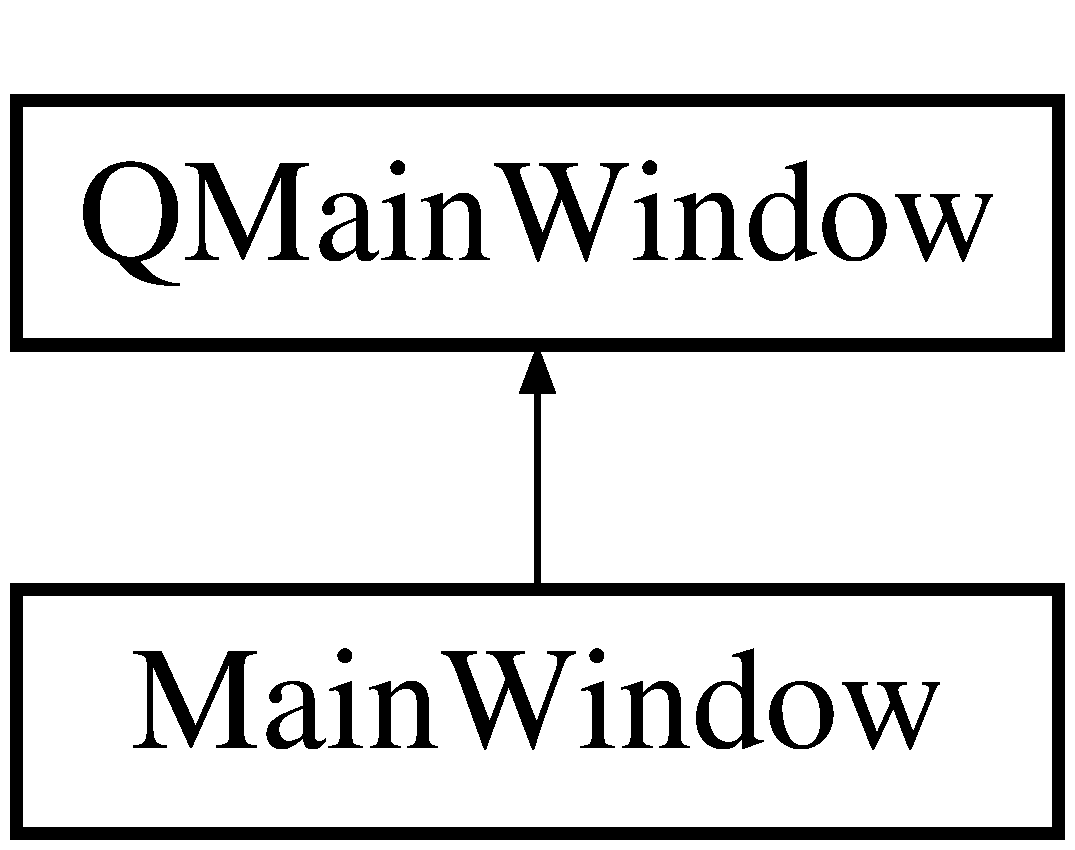
\includegraphics[height=2.000000cm]{class_main_window}
\end{center}
\end{figure}
\subsection*{Открытые члены}
\begin{DoxyCompactItemize}
\item 
\mbox{\Hypertarget{class_main_window_a8b244be8b7b7db1b08de2a2acb9409db}\label{class_main_window_a8b244be8b7b7db1b08de2a2acb9409db}} 
{\bfseries Main\+Window} (Q\+Widget $\ast$parent=0)
\end{DoxyCompactItemize}


Объявления и описания членов классов находятся в файлах\+:\begin{DoxyCompactItemize}
\item 
\mbox{\hyperlink{mainwindow_8h}{mainwindow.\+h}}\item 
\mbox{\hyperlink{mainwindow_8cpp}{mainwindow.\+cpp}}\end{DoxyCompactItemize}

\chapter{Файлы}
\hypertarget{datatable_8cpp}{}\section{Файл datatable.\+cpp}
\label{datatable_8cpp}\index{datatable.\+cpp@{datatable.\+cpp}}


Файл исходников с реализацией всех необходимых функций.  


{\ttfamily \#include $<$datatable.\+h$>$}\newline
{\ttfamily \#include $<$Q\+String$>$}\newline
{\ttfamily \#include $<$Q\+Dialog$>$}\newline
{\ttfamily \#include $<$Q\+File\+Dialog$>$}\newline
{\ttfamily \#include $<$Q\+Message\+Box$>$}\newline
{\ttfamily \#include $<$Q\+File$>$}\newline
{\ttfamily \#include $<$Q\+Text\+Stream$>$}\newline
{\ttfamily \#include $<$Q\+Text\+Codec$>$}\newline
{\ttfamily \#include $<$Qt\+Sql$>$}\newline
{\ttfamily \#include $<$Q\+Sql\+Record$>$}\newline
\subsection*{Функции}
\begin{DoxyCompactItemize}
\item 
bool \mbox{\hyperlink{datatable_8cpp_a448d6b5189991394bc06db5950f2c8dc}{operator==}} (const \mbox{\hyperlink{class_data_table}{Data\+Table}} \&L, const \mbox{\hyperlink{class_data_table}{Data\+Table}} \&R)
\end{DoxyCompactItemize}


\subsection{Подробное описание}
Файл исходников с реализацией всех необходимых функций. 



\subsection{Функции}
\mbox{\Hypertarget{datatable_8cpp_a448d6b5189991394bc06db5950f2c8dc}\label{datatable_8cpp_a448d6b5189991394bc06db5950f2c8dc}} 
\index{datatable.\+cpp@{datatable.\+cpp}!operator==@{operator==}}
\index{operator==@{operator==}!datatable.\+cpp@{datatable.\+cpp}}
\subsubsection{\texorpdfstring{operator==()}{operator==()}}
{\footnotesize\ttfamily bool operator== (\begin{DoxyParamCaption}\item[{const \mbox{\hyperlink{class_data_table}{Data\+Table}} \&}]{L,  }\item[{const \mbox{\hyperlink{class_data_table}{Data\+Table}} \&}]{R }\end{DoxyParamCaption})}


\begin{DoxyParams}{Аргументы}
{\em L} & Левая переменная \\
\hline
{\em R} & Права переменная \\
\hline
\end{DoxyParams}
\begin{DoxyReturn}{Возвращает}
Результат 
\end{DoxyReturn}

\hypertarget{datatable_8h}{}\section{Файл datatable.\+h}
\label{datatable_8h}\index{datatable.\+h@{datatable.\+h}}


Заголовочный файл с описанием основного класса проекта.  


{\ttfamily \#include $<$Q\+Object$>$}\newline
{\ttfamily \#include $<$Q\+List$>$}\newline
{\ttfamily \#include $<$Q\+Abstract\+Table\+Model$>$}\newline
{\ttfamily \#include $<$Q\+String$>$}\newline
\subsection*{Классы}
\begin{DoxyCompactItemize}
\item 
class \mbox{\hyperlink{class_data_table}{Data\+Table}}
\begin{DoxyCompactList}\small\item\em Класс \mbox{\hyperlink{class_data_table}{Data\+Table}}. Основной класс в этом проекте. \end{DoxyCompactList}\end{DoxyCompactItemize}


\subsection{Подробное описание}
Заголовочный файл с описанием основного класса проекта. 


\hypertarget{mainwindow_8cpp}{}\section{Файл mainwindow.\+cpp}
\label{mainwindow_8cpp}\index{mainwindow.\+cpp@{mainwindow.\+cpp}}


Файл исходников с описанием работы главного окна проекта.  


{\ttfamily \#include \char`\"{}mainwindow.\+h\char`\"{}}\newline
{\ttfamily \#include \char`\"{}ui\+\_\+mainwindow.\+h\char`\"{}}\newline
{\ttfamily \#include $<$Q\+Dialog$>$}\newline
{\ttfamily \#include $<$Q\+File\+Dialog$>$}\newline
{\ttfamily \#include $<$Q\+Message\+Box$>$}\newline


\subsection{Подробное описание}
Файл исходников с описанием работы главного окна проекта. 


\hypertarget{mainwindow_8h}{}\section{Файл mainwindow.\+h}
\label{mainwindow_8h}\index{mainwindow.\+h@{mainwindow.\+h}}


Заголовочный файл с описанием главного окна проекта.  


{\ttfamily \#include $<$Q\+Main\+Window$>$}\newline
{\ttfamily \#include $<$Q\+String$>$}\newline
{\ttfamily \#include $<$datatable.\+h$>$}\newline
{\ttfamily \#include $<$Q\+Standard\+Item$>$}\newline
{\ttfamily \#include $<$Q\+Standard\+Item\+Model$>$}\newline
\subsection*{Классы}
\begin{DoxyCompactItemize}
\item 
class \mbox{\hyperlink{class_main_window}{Main\+Window}}
\end{DoxyCompactItemize}


\subsection{Подробное описание}
Заголовочный файл с описанием главного окна проекта. 


%--- End generated contents ---

% Index
\backmatter
\newpage
\phantomsection
\clearemptydoublepage
\addcontentsline{toc}{chapter}{Алфавитный указатель}
\printindex

\end{document}
